\documentclass[11pt,a4paper,oneside,openany]{memoir}

% -----------------------------------------------------------------------------
% A student-facing guide to the research repository.
% Compile from the repository root with:
%   latexmk -pdf -interaction=nonstopmode -halt-on-error \
%     -output-directory=output/pdf docs/research_project_guide.tex
% -----------------------------------------------------------------------------

\usepackage[T1]{fontenc}
\usepackage{newpxtext,newpxmath}
\usepackage[a4paper,margin=24mm,headheight=15pt]{geometry}
\usepackage{microtype}
\usepackage{mathtools,bm}
\usepackage{graphicx}
\usepackage{booktabs,tabularx,array,multirow}
\usepackage{enumitem}
\usepackage{siunitx}
\usepackage{xcolor}
\usepackage{tikz}
\usetikzlibrary{arrows.meta,positioning,calc,fit,shapes.geometric,backgrounds}
\usepackage{pgfplots}
\pgfplotsset{compat=1.18}
\usepackage[most]{tcolorbox}
\usepackage{listings}
\usepackage{caption,subcaption}
\usepackage{float}
\usepackage{hyperref}
\usepackage[capitalise,noabbrev]{cleveref}

\definecolor{Ink}{HTML}{172A3A}
\definecolor{Navy}{HTML}{173F5F}
\definecolor{Teal}{HTML}{168C86}
\definecolor{Sky}{HTML}{DDF2F5}
\definecolor{Gold}{HTML}{F2B84B}
\definecolor{Orange}{HTML}{E87839}
\definecolor{Coral}{HTML}{D95D64}
\definecolor{Leaf}{HTML}{4D8B57}
\definecolor{Mist}{HTML}{F3F7F8}
\definecolor{SoftGold}{HTML}{FFF4D6}
\definecolor{SoftCoral}{HTML}{FCE8E8}
\definecolor{MidGrey}{HTML}{5D6A72}
\definecolor{LightRule}{HTML}{D6E0E4}

\hypersetup{
  colorlinks=true,
  linkcolor=Navy,
  citecolor=Teal,
  urlcolor=Orange,
  pdftitle={Random-environment dimers and spanning trees: a guided research map},
  pdfsubject={Student-facing guide to the Durham research repository},
  pdfkeywords={dimers, spanning trees, height functions, random environments, super-roughness}
}

\setsecnumdepth{subsection}
\settocdepth{section}
\setlength{\parindent}{0pt}
\setlength{\parskip}{0.55em}
\setlist{itemsep=0.25em,topsep=0.35em,leftmargin=1.65em}
\renewcommand{\arraystretch}{1.18}
\sisetup{detect-all,group-separator={,},group-minimum-digits=4}

\makepagestyle{research}
\makeevenhead{research}{\small\color{MidGrey}\leftmark}{}{\small\color{MidGrey}\thepage}
\makeoddhead{research}{\small\color{MidGrey}\leftmark}{}{\small\color{MidGrey}\thepage}
\makeevenfoot{research}{}{}{}
\makeoddfoot{research}{}{}{}
\makeheadrule{research}{\textwidth}{0.4pt}
\pagestyle{research}

\chapterstyle{hangnum}
\renewcommand{\chapnamefont}{\normalfont\large\scshape\color{Teal}}
\renewcommand{\chapnumfont}{\normalfont\fontsize{44}{46}\selectfont\bfseries\color{Gold}}
\renewcommand{\chaptitlefont}{\normalfont\huge\bfseries\color{Navy}}
\renewcommand{\printchapternum}{%
  \noindent\llap{\makebox[\chapindent][r]{\chapnumfont\thechapter\hspace{1.2em}}}}
\setbeforesecskip{-1.2\baselineskip plus -0.3\baselineskip minus -0.2\baselineskip}
\setaftersecskip{0.45\baselineskip}
\setsecheadstyle{\Large\bfseries\color{Navy}}
\setsubsecheadstyle{\large\bfseries\color{Teal}}
\setsubsubsecheadstyle{\normalsize\bfseries\color{Ink}}

\newcommand{\E}{\mathbb{E}}
\newcommand{\Var}{\operatorname{Var}}
\newcommand{\Cov}{\operatorname{Cov}}
\newcommand{\Prob}{\mathbb{P}}
\newcommand{\given}{\,\middle|\,}
\newcommand{\dd}{\,\mathrm{d}}
\newcommand{\code}[1]{\texttt{#1}}
\newcommand{\R}{\mathbb{R}}
\newcommand{\1}{\bm{1}}

\newtcolorbox{bigidea}[1]{
  enhanced,breakable,colback=Sky,colframe=Teal,boxrule=0.8pt,
  arc=2mm,left=3mm,right=3mm,top=2mm,bottom=2mm,
  title={#1},fonttitle=\bfseries\color{Navy},coltitle=Navy
}
\newtcolorbox{resultbox}[1]{
  enhanced,breakable,colback=SoftGold,colframe=Gold,boxrule=0.8pt,
  arc=2mm,left=3mm,right=3mm,top=2mm,bottom=2mm,
  title={#1},fonttitle=\bfseries\color{Ink},coltitle=Ink
}
\newtcolorbox{warningbox}[1]{
  enhanced,breakable,colback=SoftCoral,colframe=Coral,boxrule=0.8pt,
  arc=2mm,left=3mm,right=3mm,top=2mm,bottom=2mm,
  title={#1},fonttitle=\bfseries\color{Ink},coltitle=Ink
}
\newtcolorbox{practicebox}[1]{
  enhanced,breakable,colback=Mist,colframe=LightRule,boxrule=0.8pt,
  arc=2mm,left=3mm,right=3mm,top=2mm,bottom=2mm,
  title={#1},fonttitle=\bfseries\color{Navy},coltitle=Navy
}

\lstdefinelanguage{JuliaMini}{
  morekeywords={function,end,for,in,if,else,return,using,const,where,struct},
  sensitive=true,
  morecomment=[l]{\#},
  morestring=[b]"
}
\lstset{
  language=JuliaMini,
  basicstyle=\ttfamily\small,
  keywordstyle=\color{Navy}\bfseries,
  commentstyle=\color{Leaf},
  stringstyle=\color{Orange},
  backgroundcolor=\color{Mist},
  frame=single,
  rulecolor=\color{LightRule},
  breaklines=true,
  columns=fullflexible,
  xleftmargin=1mm,
  xrightmargin=1mm,
  aboveskip=0.7em,
  belowskip=0.7em
}

\captionsetup{font=small,labelfont={bf,color=Navy}}

\begin{document}

\pagenumbering{gobble}
\begin{titlingpage}
\pagecolor{Mist}
\begin{tikzpicture}[remember picture,overlay]
  \fill[Navy] (current page.north west) rectangle ([yshift=-8.2cm]current page.north east);
  \fill[Teal] ([yshift=-8.2cm]current page.north west) rectangle ([yshift=-8.45cm]current page.north east);
  \fill[Gold] ([xshift=-22mm,yshift=-18mm]current page.north east) circle (11mm);
\end{tikzpicture}

\vspace*{1.0cm}
{\color{Sky}\Large A guided map of the Durham research project\par}
\vspace{0.55cm}
{\color{white}\fontsize{32}{37}\selectfont\bfseries Random-environment dimers\\[1mm]
and spanning trees\par}
\vspace{0.55cm}
{\color{Navy}\Large\bfseries Height fluctuations, super-roughness, and what to do next\par}

\vspace{2.2cm}
\begin{center}
\begin{minipage}[t]{0.47\textwidth}
  \centering
  
\includegraphics[width=\linewidth]{aztec/results/tilings/uniform_L200.png}
  \vspace{-0.8em}
  {\small\color{MidGrey}Uniform Aztec diamond, $L=200$}
\end{minipage}\hfill
\begin{minipage}[t]{0.47\textwidth}
  \centering
  
\includegraphics[width=\linewidth]{aztec/results/tilings/gamma_disordered_L200.png}
  \vspace{-0.8em}
  {\small\color{MidGrey}Gamma-disordered Aztec diamond, $L=200$}
\end{minipage}
\end{center}

\vfill
\begin{tcolorbox}[colback=white,colframe=LightRule,boxrule=0.7pt,arc=2mm]
\textbf{Audience.} Written for a student about to begin second-year mathematics.
No prior knowledge of dimers, spanning trees, Monte Carlo, or Kasteleyn theory
is assumed. The goal is to make the project navigable without hiding the
important mathematical distinctions.
\end{tcolorbox}
\vspace{0.3cm}
{\small\color{MidGrey}Project status: 24 August 2026 \hfill Repository revision: \code{8301886}}
\end{titlingpage}
\nopagecolor

\frontmatter
\chapter*{How to use this guide}
\addcontentsline{toc}{chapter}{How to use this guide}

This document has two jobs. First, it teaches the mathematics from the ground
up. Second, it records the present state of the computational research and
turns the next scientific question into a concrete implementation plan.

If you have one hour, read the executive summary, \cref{chap:decomposition},
\cref{chap:models}, \cref{chap:results}, and \cref{chap:roadmap}. If you are
about to work on the code, also read \cref{chap:computation} and the checklist
in \cref{sec:first-implementation}.

\begin{bigidea}{The one sentence to remember}
We are testing whether randomness in the \emph{environment} creates a
$C(\log L)^2$ contribution to spatial height fluctuations, and whether the
answer depends on the geometry and on how disorder is put into the dimer
model.
\end{bigidea}

\tableofcontents*

\chapter*{Notation at a glance}
\addcontentsline{toc}{chapter}{Notation at a glance}

\begin{tabularx}{\textwidth}{>{\bfseries\color{Navy}}l X}
$L$ & Linear size or order of the finite system. Its precise geometric meaning depends on the model.\\
$\omega$ & A frozen random environment: the complete collection of random weights for one experiment.\\
$H$ & A height observable of a random tiling or matching.\\
$H_1,H_2$ & Two conditionally independent samples made in the same environment.\\
$\Delta H_a(r)$ & Spatial height increment in replica $a$ across separation $r$.\\
$T(r)$ & Conditional or connected component: $\tfrac12\Var(\Delta H_1-\Delta H_2)$.\\
$D(r)$ & Disorder component: $\Cov(\Delta H_1,\Delta H_2)$.\\
$c$ & Coefficient of $(\log L)^2$ or $(\log r)^2$ in a nested fit.\\
$K$ & A finite bipartite Kasteleyn matrix for a weighted dimer model.\\
\end{tabularx}

\mainmatter

\chapter{Executive summary}
\label{chap:summary}

The objects in this project are random domino tilings, perfect matchings,
spanning trees, and loop-erased random walks. Each object can be encoded by a
height or winding observable. The main question is how the variance of that
observable grows when the system size $L$ becomes large.

There are two competing scales:
\[
  \text{ordinary roughness: } A+B\log L,
  \qquad
  \text{super-roughness: } A+B\log L+C(\log L)^2.
\]
A positive, stable value of $C$ is the target signal. The word ``stable'' is
essential: one favourable fit at one size cutoff is not persuasive.

The crucial conceptual step was to split total randomness into two sources.
For a fixed environment $\omega$, tilings still fluctuate. In addition, the
conditional mean height changes from one environment to another. Thus
\[
\Var(H)
=\underbrace{\E_\omega[\Var(H\mid\omega)]}_{\text{conditional sampling}}
+\underbrace{\Var_\omega(\E[H\mid\omega])}_{\text{disorder background}}.
\]
Two independent replicas in the same environment let us estimate both pieces.

\begin{resultbox}{What the project currently says}
\begin{itemize}
  \item LERW winding experiments look ordinary-log-like, not super-rough.
  \item Aztec central height and same-environment height differences are not the decisive observables.
  \item In the Gamma-disordered Aztec diamond, the \emph{spatial disorder covariance} has positive finite-size quadratic-log curvature. The conditional component and uniform control do not.
  \item A structured square-grid spanning-tree/Temperley model shows no comparable robust signal up to $L=6144$, but it is not the canonical independent-edge dimer disorder.
  \item A direct independent-edge square-grid dimer model also gives a finite-size null for \emph{central height} over $L=2,\ldots,20$. A Kasteleyn replay confirms this without MCMC mixing error.
  \item Therefore the next fair comparison is direct square-grid \emph{spatial height increments}, computed deterministically with Kasteleyn correlations.
\end{itemize}
\end{resultbox}

\begin{figure}[H]
\centering
\resizebox{0.96\textwidth}{!}{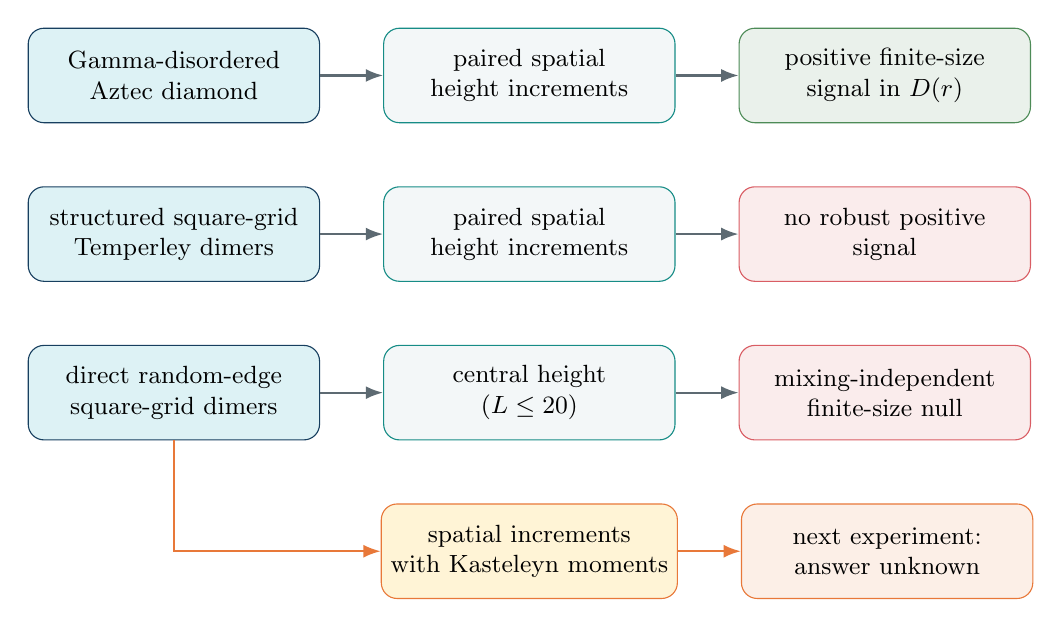
\begin{tikzpicture}[
  node distance=8mm and 8mm,
  every node/.style={font=\small,align=center},
  model/.style={rounded corners=2mm,draw=Navy,fill=Sky,minimum width=37mm,minimum height=12mm},
  obs/.style={rounded corners=2mm,draw=Teal,fill=Mist,minimum width=37mm,minimum height=12mm},
  outcome/.style={rounded corners=2mm,draw=#1,fill=#1!12,minimum width=37mm,minimum height=12mm},
  arr/.style={-{Latex[length=2.2mm]},thick,color=MidGrey}
]
\node[model] (az) {Gamma-disordered\\Aztec diamond};
\node[obs,right=of az] (azobs) {paired spatial\\height increments};
\node[outcome=Leaf,right=of azobs] (azyes) {positive finite-size\\signal in $D(r)$};

\node[model,below=of az] (temp) {structured square-grid\\Temperley dimers};
\node[obs,right=of temp] (tempobs) {paired spatial\\height increments};
\node[outcome=Coral,right=of tempobs] (tempno) {no robust positive\\signal};

\node[model,below=of temp] (direct) {direct random-edge\\square-grid dimers};
\node[obs,right=of direct] (cent) {central height\\($L\leq20$)};
\node[outcome=Coral,right=of cent] (centno) {mixing-independent\\finite-size null};

\node[obs,below=of cent,draw=Orange,fill=SoftGold] (next) {spatial increments\\with Kasteleyn moments};
\node[outcome=Orange,right=of next] (unknown) {next experiment:\\answer unknown};

\draw[arr] (az)--(azobs); \draw[arr] (azobs)--(azyes);
\draw[arr] (temp)--(tempobs); \draw[arr] (tempobs)--(tempno);
\draw[arr] (direct)--(cent); \draw[arr] (cent)--(centno);
\draw[arr,Orange] (direct.south) |- (next.west);
\draw[arr,Orange] (next)--(unknown);
\end{tikzpicture}}
\caption{The logical map of the present project. Similar words do not always mean identical models or observables.}
\label{fig:logic-map}
\end{figure}

\chapter{The mathematical objects}
\label{chap:objects}

\section{Graphs, matchings, and dimers}

A graph $G=(V,E)$ consists of vertices and edges. A \emph{matching} is a set
of edges that do not share endpoints. A \emph{perfect matching} covers every
vertex exactly once. On a square board, a domino covering two neighbouring
squares is the same thing as an edge joining their centres; a domino tiling is
therefore a perfect matching of the square-grid graph.

If every edge $e$ has a positive weight $w_e$, the weighted dimer measure is
\[
  \Prob_\omega(M)=\frac{1}{Z_\omega}\prod_{e\in M}w_e(\omega),
  \qquad
  Z_\omega=\sum_{M\text{ perfect}}\prod_{e\in M}w_e(\omega).
\]
Here $\omega$ denotes the whole weight field, not one weight. Large products
make some matchings more likely than others.

\begin{figure}[H]
\centering
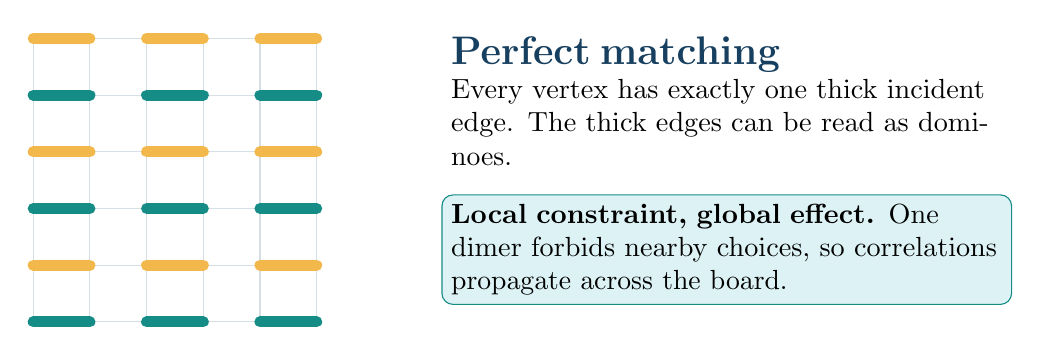
\begin{tikzpicture}[scale=0.72]
  \foreach \x in {0,...,5}{\foreach \y in {0,...,5}{\fill[Ink] (\x,\y) circle (1.5pt);}}
  \foreach \x in {0,...,4}{\foreach \y in {0,...,5}{\draw[LightRule] (\x,\y)--(\x+1,\y);}}
  \foreach \x in {0,...,5}{\foreach \y in {0,...,4}{\draw[LightRule] (\x,\y)--(\x,\y+1);}}
  \foreach \y in {0,2,4}{
    \foreach \x in {0,2,4}{\draw[line width=4pt,Teal,line cap=round] (\x,\y)--(\x+1,\y);}
  }
  \foreach \y in {1,3,5}{
    \foreach \x in {0,2,4}{\draw[line width=4pt,Gold,line cap=round] (\x,\y)--(\x+1,\y);}
  }
  \node[align=left,text width=6.3cm,anchor=north west] at (7.2,5.2) {\Large\bfseries\color{Navy} Perfect matching};
  \node[align=left,text width=7.3cm,anchor=north west] at (7.2,4.45) {Every vertex has exactly one thick incident edge. The thick edges can be read as dominoes.};
  \node[rounded corners,draw=Teal,fill=Sky,align=left,text width=7.0cm,anchor=north west] at (7.2,2.25) {\textbf{Local constraint, global effect.} One dimer forbids nearby choices, so correlations propagate across the board.};
\end{tikzpicture}
\caption{A toy square-grid perfect matching. The research uses much larger finite domains and non-uniform weights.}
\end{figure}

\section{Spanning trees and loop erasure}

A spanning tree is a connected, cycle-free set of edges touching every vertex.
On $n$ vertices it has exactly $n-1$ edges. A uniform spanning tree gives every
tree equal probability; a weighted tree gives probability proportional to the
product of its edge weights.

Wilson's algorithm samples spanning trees using loop-erased random walks.
Start a random walk from a vertex and erase loops in chronological order. Add
the remaining simple path to the growing tree, then repeat from an uncovered
vertex. This is the bridge between the project's early LERW experiments and
the later spanning-tree/Temperley experiments \cite{Wilson1996,KPW2000}.

\begin{figure}[H]
\centering
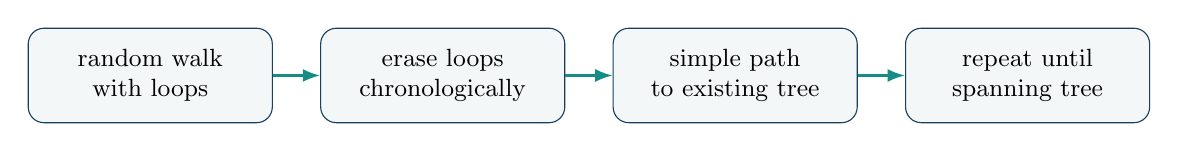
\begin{tikzpicture}[
  every node/.style={font=\small},
  stage/.style={rounded corners=2mm,draw=Navy,fill=Mist,minimum width=31mm,minimum height=12mm,align=center},
  arr/.style={-{Latex[length=2.2mm]},thick,Teal}
]
\node[stage] (walk) {random walk\\with loops};
\node[stage,right=6mm of walk] (erase) {erase loops\\chronologically};
\node[stage,right=6mm of erase] (path) {simple path\\to existing tree};
\node[stage,right=6mm of path] (tree) {repeat until\\spanning tree};
\draw[arr] (walk)--(erase); \draw[arr] (erase)--(path); \draw[arr] (path)--(tree);
\end{tikzpicture}
\caption{Wilson's algorithm in one line. The random-walk transition law can depend on a frozen environment.}
\end{figure}

\section{The height function}

A dimer height function turns a two-dimensional matching into a scalar surface
on faces. One chooses a reference face and integrates prescribed increments
while moving across edges. The local perfect-matching rule makes the sum around
every elementary loop zero, so the height is path-independent after a
convention is fixed.

In the Aztec implementation, moving down a recorded face column contributes
$+3$ across a dimer edge and $-1$ otherwise. Other orientations have compatible
sign rules. Absolute height depends on a boundary convention; a difference
$H(y)-H(x)$ is the more geometric observable.

\begin{bigidea}{Why height is useful}
A complicated tiling becomes a random surface. ``Roughness'' then means the
growth of $\Var(H(y)-H(x))$ as the separation between $x$ and $y$ grows.
The height function is not a decorative re-encoding: it is the observable
predicted to show logarithmic or quadratic-logarithmic fluctuations.
\end{bigidea}

\section{Random environments: quenched versus annealed}

An environment $\omega$ is a frozen landscape of weights. There are two
levels of randomness:

\begin{enumerate}
  \item draw the environment $\omega$;
  \item conditional on that environment, draw a tiling, matching, tree, or walk.
\end{enumerate}

\emph{Quenched} questions hold $\omega$ fixed. \emph{Annealed} questions average
over both levels. Refreshing weights at every random-walk step is a different
stochastic model: it removes the fixed spatial background and therefore cannot
support the same shared-environment covariance without a new definition.

\chapter{The key probability decomposition}
\label{chap:decomposition}

\section{The law of total variance}

Let
\[
  m(\omega)=\E[H\mid\omega],
  \qquad
  s^2(\omega)=\Var(H\mid\omega).
\]
Write $H=m(\omega)+\varepsilon$, where
$\E[\varepsilon\mid\omega]=0$. Then
\begin{align*}
\Var(H)
&=\E\bigl[(H-\E H)^2\bigr]\\
&=\E_\omega[s^2(\omega)]+\Var_\omega(m(\omega)).
\end{align*}
The cross term vanishes because the conditional mean of $\varepsilon$ is zero.

\begin{figure}[H]
\centering
\resizebox{0.96\textwidth}{!}{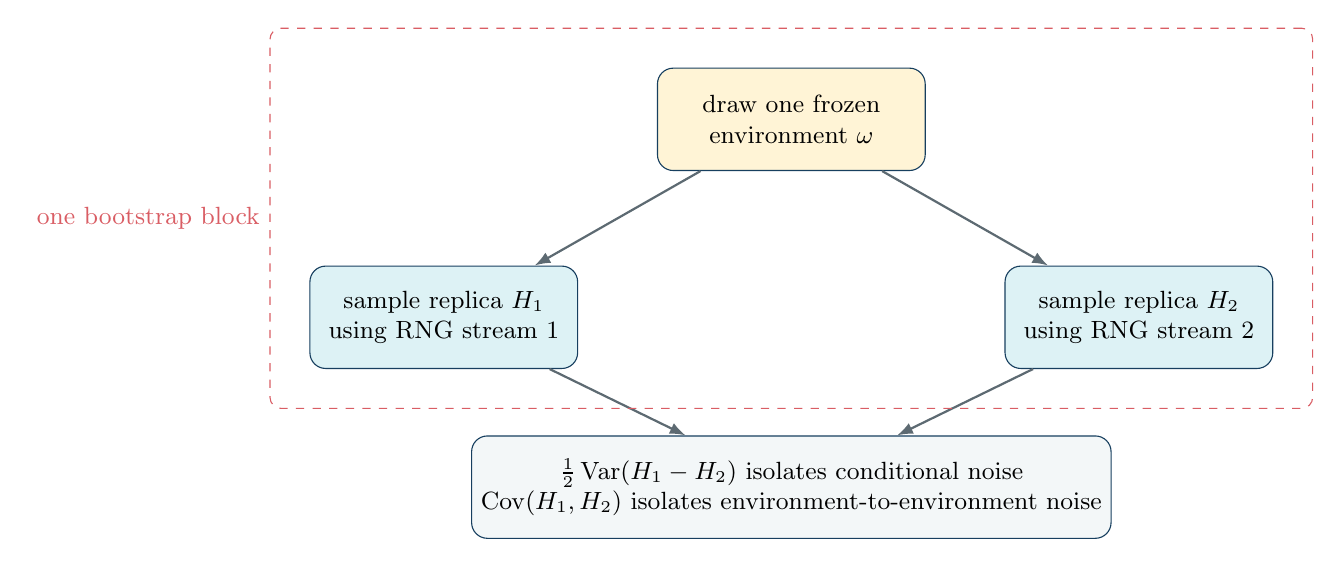
\begin{tikzpicture}[
  every node/.style={font=\small,align=center},
  box/.style={rounded corners=2mm,draw=Navy,minimum width=34mm,minimum height=13mm},
  arr/.style={-{Latex[length=2mm]},thick,MidGrey}
]
\node[box,fill=SoftGold] (omega) {draw one frozen\\environment $\omega$};
\node[box,fill=Sky,below left=12mm and 10mm of omega] (h1) {sample replica $H_1$\\using RNG stream 1};
\node[box,fill=Sky,below right=12mm and 10mm of omega] (h2) {sample replica $H_2$\\using RNG stream 2};
\node[box,fill=Mist,below=15mm of $(h1)!0.5!(h2)$,minimum width=63mm] (stats) {$\tfrac12\Var(H_1-H_2)$ isolates conditional noise\\$\Cov(H_1,H_2)$ isolates environment-to-environment noise};
\draw[arr] (omega)--(h1); \draw[arr] (omega)--(h2);
\draw[arr] (h1)--(stats); \draw[arr] (h2)--(stats);
\node[draw=Coral,dashed,rounded corners,fit=(omega)(h1)(h2),inner sep=5mm,label={[Coral]left:one bootstrap block}] {};
\end{tikzpicture}}
\caption{The paired-replica design. The replicas share $\omega$ but no conditional random choices.}
\label{fig:replicas}
\end{figure}

\section{Why two replicas recover the two pieces}

Let $H_1$ and $H_2$ be conditionally independent and identically distributed
given the same $\omega$. Conditional on $\omega$,
\[
\E[(H_1-H_2)^2\mid\omega]=2s^2(\omega),
\]
and the unconditional mean difference is zero. Hence
\[
  \boxed{\frac12\Var(H_1-H_2)=\E_\omega[s^2(\omega)]}.
\]
For the covariance, conditional independence gives
\[
\E[H_1H_2\mid\omega]=m(\omega)^2,
\]
so
\[
  \boxed{\Cov(H_1,H_2)=\Var_\omega(m(\omega))}.
\]
The replicas are independent \emph{after conditioning}, but positively
dependent marginally whenever environments shift their common mean.

\section{A complete toy example}

Suppose $\omega$ is equally likely to be A or B. In environment A, $H$ is
$-2$ or $0$ with equal probability. In B, $H$ is $0$ or $2$ with equal
probability. Then
\[
  m(A)=-1,\quad m(B)=1,\qquad s^2(A)=s^2(B)=1.
\]
Therefore
\[
  \E_\omega[s^2(\omega)]=1,
  \qquad
  \Var_\omega(m(\omega))=1,
  \qquad
  \Var(H)=2.
\]
If we draw two replicas in the same environment, direct calculation gives
$\tfrac12\Var(H_1-H_2)=1$ and $\Cov(H_1,H_2)=1$.

\begin{practicebox}{Check your understanding}
If the two replicas were accidentally given \emph{independent} environments,
their covariance would be zero. That single coding mistake would erase the
disorder component while leaving plausible-looking marginal samples.
\end{practicebox}

\section{The spatial estimands}

Choose two faces $x$ and $x+r$ and define
\[
  \Delta H_a(r)=H_a(x+r)-H_a(x),\qquad a\in\{1,2\}.
\]
The project uses
\begin{align*}
T(r)&=\frac12\Var\bigl(\Delta H_1(r)-\Delta H_2(r)\bigr),\\
D(r)&=\Cov\bigl(\Delta H_1(r),\Delta H_2(r)\bigr).
\end{align*}
Thus $T$ measures conditional tiling noise and $D$ measures how the frozen
environment moves the mean height profile. The total marginal variance is
$T(r)+D(r)$, up to the usual finite-sample estimator conventions.

\begin{warningbox}{The observable is part of the model}
Central height, winding, a two-tiling difference, and a spatial height
increment are not interchangeable. A null result for one does not logically
rule out a signal in another. This is the reason the next direct square-grid
experiment must copy the Aztec spatial observable as closely as possible.
\end{warningbox}

\chapter{Roughness and the statistical target}
\label{chap:roughness}

\section{Ordinary roughness versus super-roughness}

Set $x=\log L$. The two nested curves are
\[
  H_0:\quad y=a+bx,
  \qquad
  H_1:\quad y=a+bx+cx^2.
\]
Ordinary logarithmic growth is a straight line against $\log L$.
Super-rough growth has persistent upward curvature, represented by $c>0$.

\begin{figure}[H]
\centering
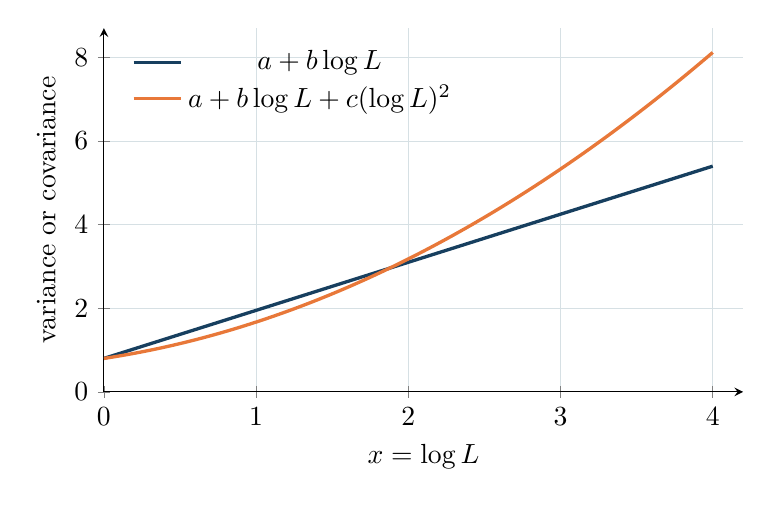
\begin{tikzpicture}
\begin{axis}[
  width=0.80\textwidth,height=6.2cm,
  axis lines=left,
  xlabel={$x=\log L$},ylabel={variance or covariance},
  xmin=0,xmax=4.2,ymin=0,ymax=8.7,
  xtick={0,1,2,3,4},ytick={0,2,4,6,8},
  grid=major,grid style={LightRule},
  legend style={draw=none,fill=none,at={(0.03,0.97)},anchor=north west}
]
\addplot[Navy,very thick,domain=0:4,samples=100]{0.8+1.15*x};
\addlegendentry{$a+b\log L$}
\addplot[Orange,very thick,domain=0:4,samples=100]{0.8+0.55*x+0.32*x^2};
\addlegendentry{$a+b\log L+c(\log L)^2$}
\end{axis}
\end{tikzpicture}
\caption{A conceptual comparison. Over a short range, the curves can be hard to distinguish; uncertainty and cutoff sensitivity matter.}
\end{figure}

The code also reports an effective power
\[
  y=C(\log L)^p.
\]
This can be descriptive, but it has no additive constant and is not the same
model as either affine fit. A fitted $p$ should not be used as a substitute for
the nested coefficient $c$.

\section{How the project evaluates a signal}

A scientifically persuasive positive result should survive several tests:

\begin{enumerate}
  \item the interval for $c$ should exclude zero in a predeclared primary fit;
  \item the sign should be stable across reasonable lower-size cutoffs;
  \item weighted and unweighted fits should tell a compatible story;
  \item the quadratic model should improve prediction on held-out large sizes;
  \item the effect should live in the predicted component, not everywhere;
  \item a no-disorder control should not produce the same effect.
\end{enumerate}

The reported convention is
\[
  \Delta\mathrm{BIC}=\mathrm{BIC}(\text{log})-\mathrm{BIC}(\text{quadratic log}).
\]
Positive values favour the extra quadratic term. These BIC values are
diagnostics from fits to noisy size-level estimates, not likelihoods fitted to
every raw height.

\section{Why the bootstrap unit is the environment}

Every observable and replica sharing one $\omega$ is dependent. Resampling
individual rows as if independent would create fictitious information.
The correct bootstrap resamples whole environments within each size, keeping
both replicas and every separation together. When four separation fractions
are pooled, their within-environment dependence must remain intact.

\chapter{The three main model families}
\label{chap:models}

\section{Gamma-disordered Aztec diamonds}

An order-$L$ Aztec diamond is tiled by dominoes. The implementation follows
the Gamma-disordered construction of Duits and Van Peski
\cite{DuitsVanPeski2025}. Two independent arrays are drawn,
\[
  a_{ij}\sim\operatorname{Gamma}(\alpha,1),\qquad
  b_{ij}\sim\operatorname{Gamma}(\beta,1),
\]
with the original experiment using $(\alpha,\beta)=(0.2,0.25)$ and the other
two weight families fixed to one by the model's convention.

Domino shuffling grows a tiling through deletion, sliding, and creation. A
Gamma-specific weight reduction supplies the creation probabilities at every
level. For two replicas, the costly reduced environment is shared but the
Bernoulli creation decisions are independent.

\begin{figure}[H]
\centering
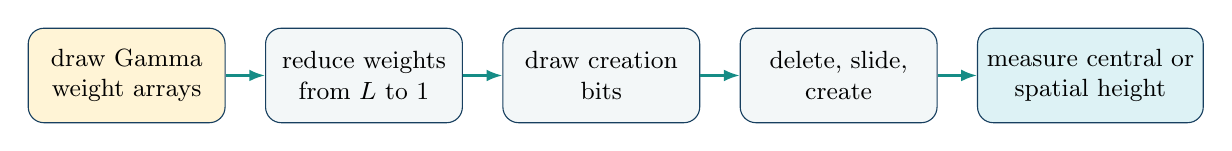
\begin{tikzpicture}[
  every node/.style={font=\small,align=center},
  stage/.style={rounded corners=2mm,draw=Navy,fill=Mist,minimum width=25mm,minimum height=12mm},
  arr/.style={-{Latex[length=2mm]},thick,Teal}
]
\node[stage,fill=SoftGold] (w) {draw Gamma\\weight arrays};
\node[stage,right=5mm of w] (r) {reduce weights\\from $L$ to $1$};
\node[stage,right=5mm of r] (c) {draw creation\\bits};
\node[stage,right=5mm of c] (s) {delete, slide,\\create};
\node[stage,right=5mm of s,fill=Sky] (h) {measure central or\\spatial height};
\draw[arr] (w)--(r); \draw[arr] (r)--(c); \draw[arr] (c)--(s); \draw[arr] (s)--(h);
\end{tikzpicture}
\caption{The Aztec production pipeline. The optimized sampler uses rolling weight buffers and packed creation bits.}
\end{figure}

For one order-$L$ tiling, runtime is $O(L^3)$, floating-point working storage
is $O(L^2)$, and stored creation decisions use $O(L^3)$ bits. The retained
spatial experiment uses symmetric central-row separations
\[
  r/L\in\{1/32,1/16,1/8,1/4\}.
\]

\section{Structured square-grid Temperley dimers}

The square-grid spanning-tree route begins with the interior lattice
\[
  \Lambda_L=\{(x,y)\in\mathbb{Z}^2:\max(|x|,|y|)<L\}
\]
and wires boundary exits to a root. Wilson's algorithm samples a weighted tree
oriented to that root. The complementary dual tree then produces a generalized
Temperley perfect matching \cite{KPW2000}.

\begin{figure}[H]
\centering
\resizebox{0.94\textwidth}{!}{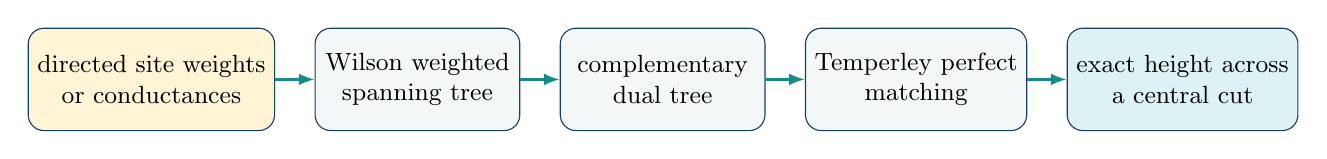
\begin{tikzpicture}[
  every node/.style={font=\small,align=center},
  stage/.style={rounded corners=2mm,draw=Navy,fill=Mist,minimum width=26mm,minimum height=13mm},
  arr/.style={-{Latex[length=2mm]},thick,Teal}
]
\node[stage,fill=SoftGold] (env) {directed site weights\\or conductances};
\node[stage,right=5mm of env] (tree) {Wilson weighted\\spanning tree};
\node[stage,right=5mm of tree] (dual) {complementary\\dual tree};
\node[stage,right=5mm of dual] (match) {Temperley perfect\\matching};
\node[stage,right=5mm of match,fill=Sky] (height) {exact height across\\a central cut};
\draw[arr] (env)--(tree); \draw[arr] (tree)--(dual); \draw[arr] (dual)--(match); \draw[arr] (match)--(height);
\end{tikzpicture}}
\caption{The structured square-grid route. The matching weights inherit a special structure from the tree construction.}
\end{figure}

The directed site-i.i.d. model assigns four outgoing weights at each site;
opposite orientations of one geometric edge need not agree. An undirected
conductance version is a separate model. Both give valid weighted Temperley
dimers, but neither is automatically the canonical random-bond dimer model
with independent weights on every dimer edge.

\begin{warningbox}{Why the structured null is not the final answer}
The large $L\leq6144$ campaign tested a genuine dimer measure, but a structured
one inherited from a spanning tree. Its null result applies to that law. It
does not by itself contradict an Aztec result or settle the independent-edge
square-lattice dimer question.
\end{warningbox}

\section{Direct random-edge square-grid dimers}

The direct model uses a tileable $2L\times2L$ square. Every dimer edge receives
an independent positive mean-one weight. The production Gamma law uses shape
$k=0.5$ and scale $1/k=2$. This is deliberately independent of the
spanning-tree/Temperley construction.

There are two computational routes to the same finite-volume Gibbs measure.

\subsection{Local heat-bath Glauber dynamics}

Choose a face uniformly. If two opposite dimers occupy it, denote the four
clockwise edge weights by $(a,b,c,d)$. Replace the pair by the top-bottom
orientation with probability
\[
  \frac{ac}{ac+bd},
\]
and by the left-right orientation with probability $bd/(ac+bd)$.

\begin{figure}[H]
\centering
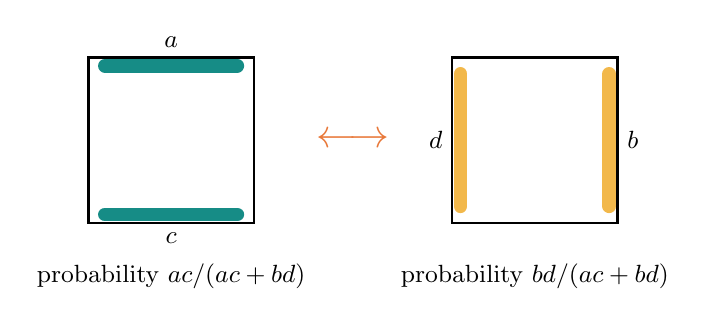
\begin{tikzpicture}[scale=1.05,every node/.style={font=\small}]
\begin{scope}
  \draw[thick] (0,0) rectangle (2,2);
  \draw[Teal,line width=5pt,line cap=round] (0.2,1.9)--(1.8,1.9);
  \draw[Teal,line width=5pt,line cap=round] (0.2,0.1)--(1.8,0.1);
  \node[above] at (1,2) {$a$}; \node[below] at (1,0) {$c$};
  \node at (1,-0.65) {probability $ac/(ac+bd)$};
\end{scope}
\node[font=\Large\bfseries\color{Orange}] at (3.2,1) {$\longleftrightarrow$};
\begin{scope}[xshift=4.4cm]
  \draw[thick] (0,0) rectangle (2,2);
  \draw[Gold,line width=5pt,line cap=round] (0.1,0.2)--(0.1,1.8);
  \draw[Gold,line width=5pt,line cap=round] (1.9,0.2)--(1.9,1.8);
  \node[left] at (0,1) {$d$}; \node[right] at (2,1) {$b$};
  \node at (1,-0.65) {probability $bd/(ac+bd)$};
\end{scope}
\end{tikzpicture}
\caption{The local weighted dimer heat bath. Non-flippable faces create self-loops.}
\end{figure}

The implementation includes exact self-loop skipping and parallel tempering.
Two chains start from opposite extremal height configurations. Agreement of
their retained summaries, effective sample size, and exchange diagnostics are
mixing checks, not proofs of mixing.

\subsection{Finite Kasteleyn calculation}

For a finite planar bipartite graph, a signed or phased weighted adjacency
matrix $K$ can encode the dimer partition function. In this project horizontal
entries are real and vertical entries carry the phase $i$. Then
\[
  Z_\omega=|\det K_\omega|.
\]
Selected entries of $K_\omega^{-1}$ give edge-occupation probabilities and
covariances \cite{Kasteleyn1961,Kenyon2009}. A height difference along a dual
path is a linear combination
\[
  X=x_0+\sum_{e\text{ crossed}}q_e\1_{\{e\text{ occupied}\}},
\]
so $\E[X\mid\omega]$ and $\Var(X\mid\omega)$ follow directly from those edge
moments.

\begin{bigidea}{Why Kasteleyn is decisive here}
The answer for a fixed finite environment is deterministic up to numerical
linear algebra. There is no burn-in, autocorrelation, or replica-flow question.
The exact replay can use precisely the same environment seeds as the MCMC
campaign, making environment-by-environment comparisons possible.
\end{bigidea}

The current dense matrix has order $2L^2$. Dense factorization therefore has
roughly cubic cost in the matrix order, which grows like $L^6$ in time and
$L^4$ in memory. This is why a spatial size benchmark must precede a larger
campaign, and why sparse or nested-dissection methods may become necessary.

\chapter{Computation, data, and reproducibility}
\label{chap:computation}

\section{Repository architecture}

The active package is dependency-light Julia. Mathematical kernels live in
three modules; scripts handle campaigns and analysis.

\begin{figure}[H]
\centering
\resizebox{0.84\textwidth}{!}{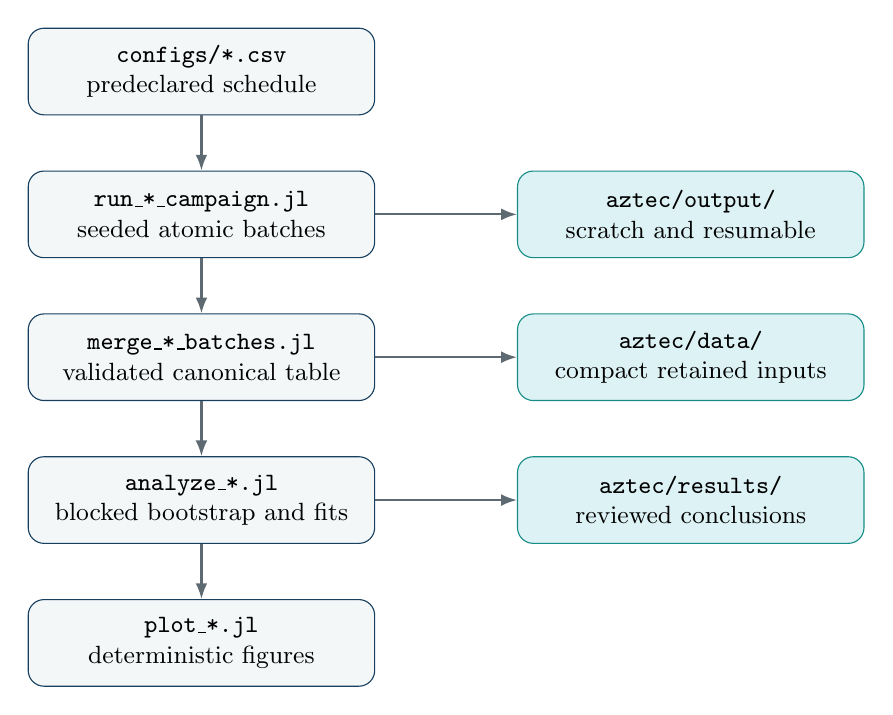
\begin{tikzpicture}[
  node distance=7mm,
  every node/.style={font=\small,align=center},
  pipe/.style={rounded corners=2mm,draw=Navy,fill=Mist,minimum width=44mm,minimum height=11mm},
  data/.style={rounded corners=2mm,draw=Teal,fill=Sky,minimum width=44mm,minimum height=11mm},
  arr/.style={-{Latex[length=2mm]},thick,MidGrey}
]
\node[pipe] (config) {\code{configs/*.csv}\\predeclared schedule};
\node[pipe,below=of config] (run) {\code{run\_*\_campaign.jl}\\seeded atomic batches};
\node[pipe,below=of run] (merge) {\code{merge\_*\_batches.jl}\\validated canonical table};
\node[pipe,below=of merge] (an) {\code{analyze\_*.jl}\\blocked bootstrap and fits};
\node[pipe,below=of an] (plot) {\code{plot\_*.jl}\\deterministic figures};
\node[data,right=18mm of run] (out) {\code{aztec/output/}\\scratch and resumable};
\node[data,right=18mm of merge] (ret) {\code{aztec/data/}\\compact retained inputs};
\node[data,right=18mm of an] (res) {\code{aztec/results/}\\reviewed conclusions};
\draw[arr] (config)--(run); \draw[arr] (run)--(merge); \draw[arr] (merge)--(an); \draw[arr] (an)--(plot);
\draw[arr] (run)--(out); \draw[arr] (merge)--(ret); \draw[arr] (an)--(res);
\end{tikzpicture}}
\caption{The data flow. Large raw HPC traces remain outside Git but are represented by configs, metadata, manifests, checksums, and compact tables.}
\end{figure}

\begin{tabularx}{\textwidth}{>{\ttfamily\color{Navy}}l X}
aztec/src/AztecDiamond.jl & Gamma-disordered domino shuffling and Aztec height observables.\\
aztec/src/SquareGrid.jl & Weighted Wilson trees, dual trees, Temperley matchings, and spatial heights.\\
aztec/src/GlauberSquareGrid.jl & Direct dimer heat bath, exact enumeration, tempering, and Kasteleyn moments.\\
docs/RESULTS.md & Chronological numerical ledger and qualifications.\\
docs/ROADMAP.md & Current ordered scientific plan and decision gates.\\
\end{tabularx}

\section{Deterministic seeds and atomic output}

Observation seeds are deterministic functions of the campaign seed, model
parameters, $L$, environment identifier, and replica identifier. Therefore
thread scheduling and batch size cannot change a scientific sample.

Runners first write temporary batches and rename them only after validation.
On restart, existing schema, row counts, identifiers, and seeds are checked
before a batch is skipped. A malformed batch stops the run rather than being
silently overwritten.

\section{Verification ladder}

\begin{enumerate}
  \item exhaustive enumeration and detailed balance on tiny state spaces;
  \item structural invariants for tilings, trees, matchings, and heights;
  \item reference-versus-optimized comparisons;
  \item deterministic seed replay and collision checks;
  \item end-to-end command-line smoke workflows;
  \item production diagnostics, blocked bootstrap, and negative controls.
\end{enumerate}

For the direct Kasteleyn method, $L=1,2$ weighted partition functions and
central-height moments agree with enumeration to about $10^{-12}$. Of 960
production environments, one ill-conditioned $L=12$ case automatically used
256-bit arithmetic; the maximum retained solve residual was
$7.39\times10^{-12}$.

\section{Running the tests}

\begin{lstlisting}[language=bash]
julia --project=aztec -e 'using Pkg; Pkg.test()'
sh aztec/test/smoke_workflows.sh
\end{lstlisting}

These commands test mathematical kernels and public workflows. They do not
regenerate the large Hamilton campaigns.

\chapter{What has been tried and what was learned}
\label{chap:results}

\section{Research timeline}

\begin{figure}[H]
\centering
\resizebox{0.96\textwidth}{!}{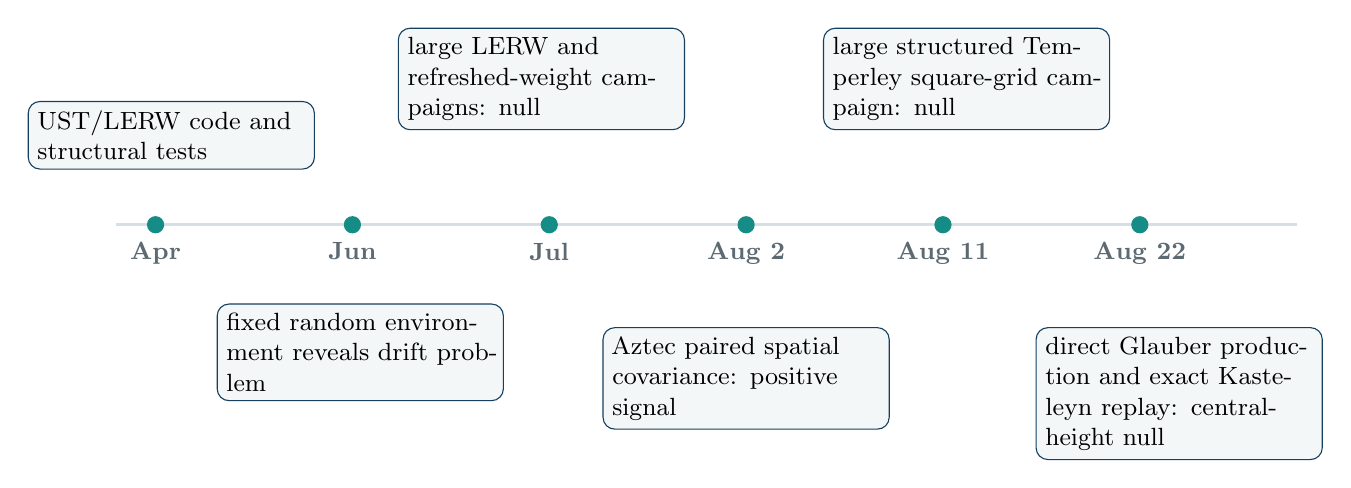
\begin{tikzpicture}[
  x=1cm,y=1cm,
  event/.style={rounded corners=1.5mm,draw=Navy,fill=Mist,text width=3.4cm,align=left,font=\small},
  dot/.style={circle,fill=Teal,inner sep=2.2pt}
]
\draw[very thick,LightRule] (0,0)--(15,0);
\foreach \x/\lab in {0.5/Apr,3/Jun,5.5/Jul,8/Aug 2,10.5/Aug 11,13/Aug 22}{
  \node[dot] at (\x,0) {};
  \node[below=3pt,font=\small\bfseries\color{MidGrey}] at (\x,0) {\lab};
}
\node[event,above=7mm] at (0.7,0) {UST/LERW code and structural tests};
\node[event,below=10mm] at (3.1,0) {fixed random environment reveals drift problem};
\node[event,above=12mm] at (5.4,0) {large LERW and refreshed-weight campaigns: null};
\node[event,below=13mm] at (8.0,0) {Aztec paired spatial covariance: positive signal};
\node[event,above=12mm] at (10.8,0) {large structured Temperley square-grid campaign: null};
\node[event,below=13mm] at (13.5,0) {direct Glauber production and exact Kasteleyn replay: central-height null};
\end{tikzpicture}}
\caption{The project evolved by repairing model and observable mismatches, not by repeating one calculation.}
\end{figure}

\section{Condensed evidence table}

\small
\begin{tabularx}{\textwidth}{>{\raggedright\arraybackslash}p{0.19\textwidth} >{\raggedright\arraybackslash}p{0.19\textwidth} >{\raggedright\arraybackslash}p{0.21\textwidth} X}
\toprule
\textbf{Model} & \textbf{Scale and data} & \textbf{Observable} & \textbf{Finding}\\
\midrule
LERW, many disorder laws & 379,000 independent environments; to $L=8192$ for key laws & winding variance and paired differences & effective powers about $1.01$--$1.19$; ordinary log generally preferred\\
Refreshed-weight LERW & about 46,000 runs; to $L=8192$ in an extension & winding and length & winding ordinary-log-like; length exponent $1.2518$, consistent with $5/4$\\
Aztec Gamma & 35,536 samples; to $L=1300$ & central height & not a convincing $p=2$ diagnostic\\
Aztec Gamma pairs & 28,304 environments & central-height difference & conditional component ordinary-log-like\\
Aztec Gamma spatial & 6,900 environments, plus 5,500 uniform controls & $T(r)$ and $D(r)$ at four fractions & positive quadratic-log curvature in $D(r)$; not in $T(r)$ or control\\
Structured Temperley square grid & five disorder laws; to $L=6144$ & paired spatial height & no robust positive coefficient; model-scope caveat\\
Direct square-grid Gamma & 960 environments; $L=2$--20 & central-height components & finite-size null in Glauber and exact Kasteleyn analyses\\
\bottomrule
\end{tabularx}
\normalsize

\section{The strongest positive evidence: Aztec spatial covariance}

The joint Gamma analysis pools four relative separations while giving each its
own intercept and log slope. One common $c$ captures quadratic-log curvature.
Whole environments are bootstrapped jointly.

\begin{resultbox}{Primary Aztec spatial result}
Unweighted: $c=0.584$, 95\% interval $[0.196,0.952]$,
$\Prob(c>0)=99.88\%$, and $\Delta\mathrm{BIC}=10.85$.
The held-out RMSE improves from $0.886$ to $0.588$.

Inverse-variance weighted: $c=0.495$, interval $[0.193,0.798]$,
$\Delta\mathrm{BIC}=14.57$, and held-out RMSE improves from $1.026$ to $0.608$.
\end{resultbox}

\begin{figure}[H]
\centering

\includegraphics[width=0.96\textwidth]{aztec/results/spatial/pooled_log2_coefficients.png}
\caption{The pooled quadratic-log coefficient. Only the Gamma disorder covariance is clearly positive. Blue is unweighted and orange is precision-weighted.}
\label{fig:pooled-coeff}
\end{figure}

\begin{figure}[H]
\centering

\includegraphics[width=0.96\textwidth]{aztec/results/spatial/spatial_variance_decomposition.png}
\caption{Aztec spatial variance decomposition at separation $L/4$. The black total is the sum of blue conditional and orange disorder components; green is the uniform control.}
\label{fig:spatial-decomp}
\end{figure}

\begin{figure}[H]
\centering
\begin{subfigure}[t]{0.49\textwidth}
\centering

\includegraphics[width=\linewidth]{aztec/results/spatial/gamma_disorder_spatial_fits.png}
\caption{Gamma disorder covariance fits.}
\end{subfigure}\hfill
\begin{subfigure}[t]{0.49\textwidth}
\centering

\includegraphics[width=\linewidth]{aztec/results/spatial/uniform_control_spatial_fits.png}
\caption{Uniform negative control fits.}
\end{subfigure}
\caption{The positive curvature is model- and component-specific, rather than an artefact automatically generated by the fitting pipeline.}
\end{figure}

At individual fractions the fitted $c$ values are $0.566$, $0.338$, $1.045$,
and $0.389$ for $1/32$, $1/16$, $1/8$, and $1/4$. Only two individual
intervals exclude zero, which is why the environment-clustered joint analysis
is important. The project interprets this as finite-size evidence, not an
asymptotic theorem.

\section{Why central height was not enough}

The single-height data contain 35,536 environments, yet total central variance
mixes conditional and disorder sources. The paired central-height analysis
improved interpretation: the difference behaved ordinary-log-like, while the
covariance curved upward but became imprecise at higher cutoffs. Spatial
increments then produced the clearest component-specific test.

\begin{figure}[H]
\centering
\begin{subfigure}[t]{0.32\textwidth}
\centering

\includegraphics[width=\linewidth]{aztec/results/height/center_height_variance.png}
\caption{Single central height.}
\end{subfigure}\hfill
\begin{subfigure}[t]{0.32\textwidth}
\centering

\includegraphics[width=\linewidth]{aztec/results/double_dimer/variance_decomposition.png}
\caption{Paired decomposition.}
\end{subfigure}\hfill
\begin{subfigure}[t]{0.32\textwidth}
\centering

\includegraphics[width=\linewidth]{aztec/results/double_dimer/disorder_covariance_fits.png}
\caption{Disorder covariance.}
\end{subfigure}
\caption{The history of the Aztec observable: total central height, component decomposition, then the more informative spatial experiment.}
\end{figure}

\section{The structured square-grid null}

The completed Temperley campaign covered five structured disorder laws and
three fitting windows. Fourteen of fifteen intervals for the quadratic term
contained zero, and fourteen of fifteen BIC comparisons preferred ordinary
log. The no-disorder control was consistent with zero. This is strong evidence
for those particular structured laws, not for every square-grid dimer law.

\section{The direct square-grid central-height null}

The Glauber production used 960 frozen Gamma environments and 352 all-one
controls. Each environment supplied two extremal-start chains with 2,000
retained heights. Mixing concerns appeared at $L=16,20$, so every Gamma
environment was replayed with finite Kasteleyn moments.

\begin{figure}[H]
\centering
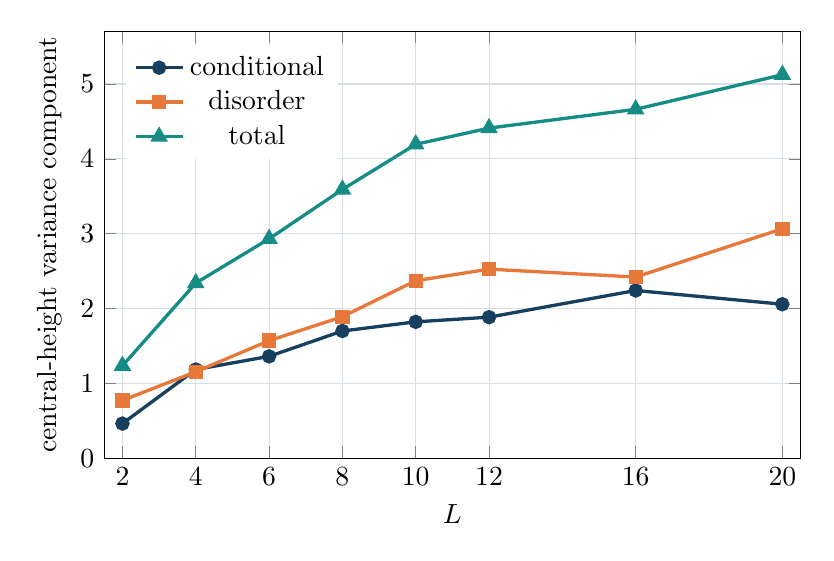
\begin{tikzpicture}
\begin{axis}[
  width=0.86\textwidth,height=7cm,
  xlabel={$L$},ylabel={central-height variance component},
  xmin=1.5,xmax=20.5,ymin=0,ymax=5.7,
  xtick={2,4,6,8,10,12,16,20},
  grid=major,grid style={LightRule},
  legend style={draw=none,fill=white,at={(0.03,0.97)},anchor=north west}
]
\addplot[Navy,very thick,mark=*,mark size=2pt] coordinates {
  (2,0.4631)(4,1.1851)(6,1.3609)(8,1.6999)(10,1.8220)(12,1.8846)(16,2.2411)(20,2.0574)};
\addlegendentry{conditional}
\addplot[Orange,very thick,mark=square*,mark size=2pt] coordinates {
  (2,0.7723)(4,1.1548)(6,1.5707)(8,1.8908)(10,2.3719)(12,2.5262)(16,2.4207)(20,3.0663)};
\addlegendentry{disorder}
\addplot[Teal,very thick,mark=triangle*,mark size=2.5pt] coordinates {
  (2,1.2355)(4,2.3399)(6,2.9315)(8,3.5907)(10,4.1939)(12,4.4108)(16,4.6618)(20,5.1237)};
\addlegendentry{total}
\end{axis}
\end{tikzpicture}
\caption{Exact Kasteleyn component estimates for the direct square-grid central height. Total equals conditional plus disorder.}
\label{fig:kasteleyn-components}
\end{figure}

For the primary full-range exact fit:

\begin{center}
\begin{tabular}{lrrrr}
\toprule
\textbf{Component} & $c$ & \textbf{95\% interval} & $\Delta$BIC & \textbf{LOOCV RMSE log / quad.}\\
\midrule
Conditional & $-0.145$ & $[-0.379,0.090]$ & $2.454$ & $0.179/0.145$\\
Disorder & $0.130$ & $[-0.552,0.785]$ & $-0.625$ & $0.241/0.283$\\
Total & $-0.015$ & $[-0.801,0.714]$ & $-2.046$ & $0.145/0.251$\\
\bottomrule
\end{tabular}
\end{center}

The conditional quadratic fit receives modest BIC support, but its coefficient
is negative and its interval includes zero. No component provides evidence for
a positive super-rough term. This is a finite-size null over $L=2$--20, not a
proof of asymptotic ordinary-log behaviour.

\section{Established, suggested, and unknown}

\begin{tabularx}{\textwidth}{>{\bfseries\color{Leaf}}p{0.17\textwidth} X}
Well supported & Ordinary-log-like behaviour for the investigated LERW winding observables; no quadratic-log signal in the Aztec conditional component; positive finite-size curvature in Aztec spatial disorder covariance for the original and stronger Gamma laws; direct square-grid central-height null over the tested finite range.\\
\end{tabularx}
\vspace{0.4em}
\begin{tabularx}{\textwidth}{>{\bfseries\color{Orange}}p{0.17\textwidth} X}
Suggested & The environment-induced background is the component capable of carrying the Aztec signal; geometry, boundary, disorder structure, or finite-size window may explain cross-model differences.\\
\end{tabularx}
\vspace{0.4em}
\begin{tabularx}{\textwidth}{>{\bfseries\color{Coral}}p{0.17\textwidth} X}
Unknown & Whether a positive $c$ persists asymptotically; whether it is universal across disorder laws; whether direct square-grid spatial disorder covariance behaves like Aztec; how large a square-grid scaling window can be reached deterministically.\\
\end{tabularx}

\chapter{The next research programme}
\label{chap:roadmap}

\begin{bigidea}{Current objective}
Run a like-for-like direct square-grid spatial-height experiment using
finite-volume Kasteleyn moments. Do not spend the next large compute allocation
on more central-height MCMC samples.
\end{bigidea}

\section{Decision-gated roadmap}

\begin{figure}[H]
\centering
\resizebox{0.90\textwidth}{!}{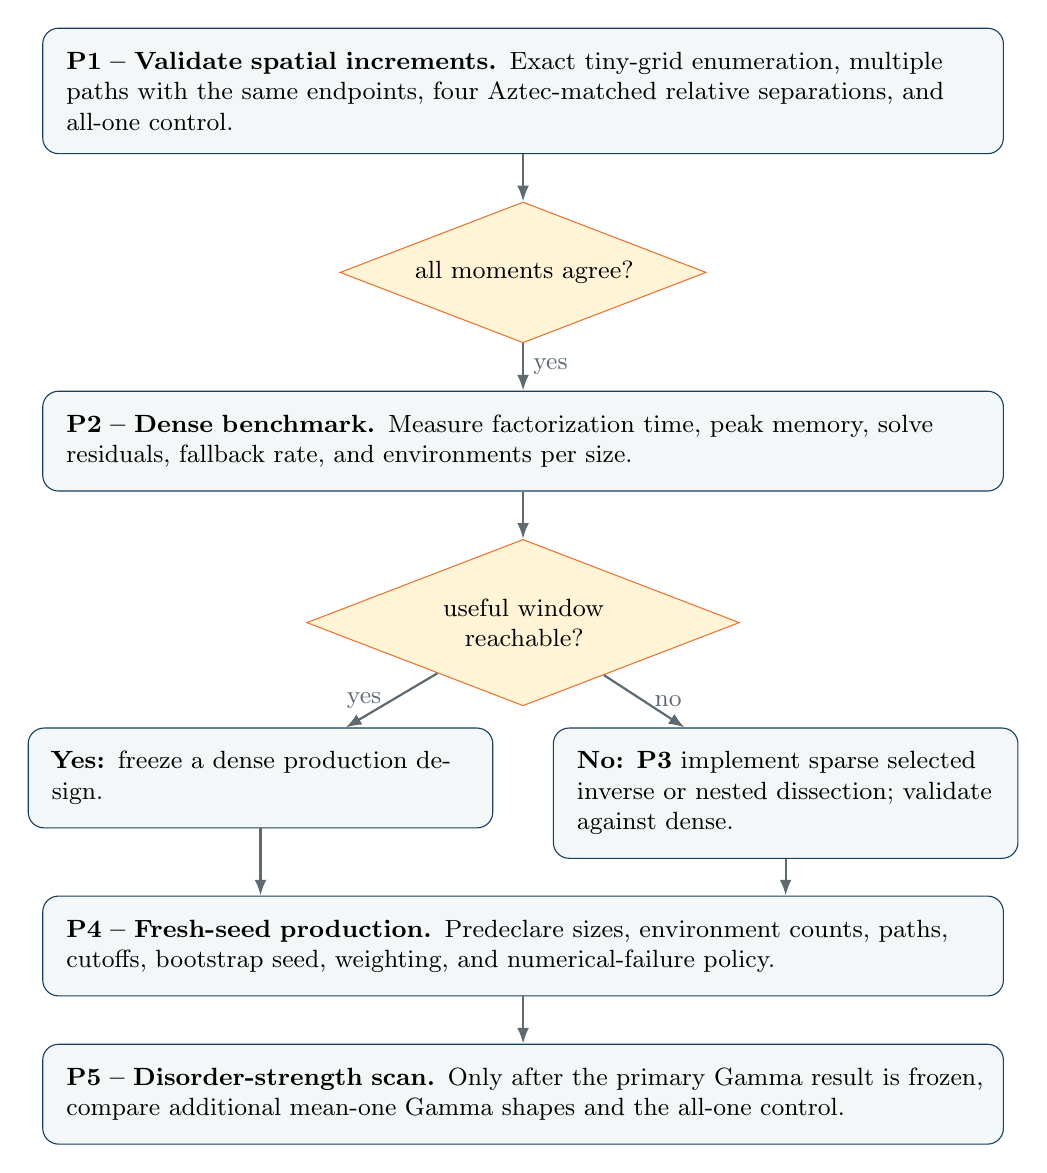
\begin{tikzpicture}[
  node distance=6mm,
  every node/.style={font=\small,align=left},
  roadstep/.style={rounded corners=2mm,draw=Navy,fill=Mist,text width=11.6cm,minimum height=12mm,inner sep=3mm},
  gate/.style={diamond,draw=Orange,fill=SoftGold,aspect=2.6,text width=3.2cm,align=center,inner sep=1mm},
  arr/.style={-{Latex[length=2mm]},thick,MidGrey}
]
\node[roadstep] (p1) {\textbf{P1 -- Validate spatial increments.} Exact tiny-grid enumeration, multiple paths with the same endpoints, four Aztec-matched relative separations, and all-one control.};
\node[gate,below=of p1] (g1) {all moments agree?};
\node[roadstep,below=of g1] (p2) {\textbf{P2 -- Dense benchmark.} Measure factorization time, peak memory, solve residuals, fallback rate, and environments per size.};
\node[gate,below=of p2] (g2) {useful window reachable?};
\node[roadstep,below left=8mm and -10mm of g2,text width=5.3cm] (p3a) {\textbf{Yes:} freeze a dense production design.};
\node[roadstep,below right=8mm and -10mm of g2,text width=5.3cm] (p3b) {\textbf{No: P3} implement sparse selected inverse or nested dissection; validate against dense.};
\node[roadstep] (p4) at ($(p3a.south)!0.5!(p3b.south)+(0,-13mm)$) {\textbf{P4 -- Fresh-seed production.} Predeclare sizes, environment counts, paths, cutoffs, bootstrap seed, weighting, and numerical-failure policy.};
\node[roadstep,below=of p4] (p5) {\textbf{P5 -- Disorder-strength scan.} Only after the primary Gamma result is frozen, compare additional mean-one Gamma shapes and the all-one control.};
\draw[arr] (p1)--(g1); \draw[arr] (g1)--node[right]{yes} (p2); \draw[arr] (p2)--(g2);
\draw[arr] (g2)--node[left]{yes} (p3a); \draw[arr] (g2)--node[right]{no} (p3b);
\draw[arr] (p3a.south) -- (p3a.south |- p4.north);
\draw[arr] (p3b.south) -- (p3b.south |- p4.north);
\draw[arr] (p4)--(p5);
\end{tikzpicture}}
\caption{The next work should proceed through validation and performance gates.}
\label{fig:roadmap}
\end{figure}

\section{P1: validate direct spatial height increments}
\label{sec:first-implementation}

The mathematical kernel already exists:
\begin{center}\code{height\_difference\_moments\_kasteleyn(weights,path)}\end{center}
A path is a
nearest-neighbour list of entries in the $(2L+1)\times(2L+1)$ height matrix.
It returns the exact conditional mean and variance plus numerical diagnostics.

The first implementation should add a multi-path spatial interface rather
than calling the present function four times independently. One Kasteleyn
factorization should be reused for every path in an environment.

\subsection{Geometry contract}

Use the same relative fractions as the Aztec and structured square-grid runs:
\[
  \rho\in\{1/32,1/16,1/8,1/4\},
  \qquad r_L(\rho)=\operatorname{round}(2L\rho).
\]
For the direct $2L\times2L$ board, choose a central height row and symmetric
endpoints. Record the exact row, start column, end column, and integer $r$ in
every retained row. Reject sizes where rounding gives $r=0$ or duplicates two
fractions.

For each endpoint pair, compare at least:

\begin{itemize}
  \item the straight central-row path;
  \item a one-row rectangular detour above;
  \item where the boundary permits, the matching detour below.
\end{itemize}

The conditional mean must agree across paths and the variance must agree
within a tolerance scaled to the solve residual. Reversing a path should
negate its mean and preserve its variance.

\subsection{Tiny-grid oracle}

For $L=1,2$, enumerate every tiling under several non-uniform environments.
For each path, calculate the height difference in every state and form the
weighted exact distribution. Compare its mean and variance with Kasteleyn
output. Also test the all-one environment. The gate is agreement at roughly
$10^{-11}$ to $10^{-12}$ in Float64 for well-conditioned examples.

\subsection{Suggested output schema}

One environment is the independent block. A long table may contain one row per
triple consisting of $L$, environment, and $\rho$, provided validation enforces that all requested
fractions are present together:

\begin{lstlisting}[language={}]
campaign_id,L,environment_id,environment_seed,
fraction_numerator,fraction_denominator,separation,
start_row,start_column,end_row,end_column,path_id,
conditional_mean,conditional_variance,
matrix_order,precision_bits,crossed_edges,
relative_solve_residual,elapsed_seconds
\end{lstlisting}

During bootstrap, resample environment identifiers and take every fraction
from the selected environment. Never resample the long rows independently.

\subsection{Code changes in order}

\begin{enumerate}
  \item Add a tested path constructor and endpoint contract in
  \code{GlauberSquareGrid.jl}.
  \item Refactor the Kasteleyn work into ``factor once, query many paths.''
  Collect the union of crossed edges and solve only the required inverse columns.
  \item Extend exact-enumeration tests to spatial differences, path reversal,
  and path independence.
  \item Add a dedicated spatial Kasteleyn runner and tiny smoke config. Keep
  the central runner's schema stable for reproducibility.
  \item Add strict restart validation: path geometry, fraction set, environment
  seed, row count, and numerical diagnostics.
  \item Extend the existing spatial analysis so conditional means supply the
  disorder component, conditional variances supply $T(r)$, and whole
  environments remain the bootstrap block.
\end{enumerate}

\begin{warningbox}{Do not manufacture replicas}
The determinantal method already gives $m_\omega(r)$ and $s^2_\omega(r)$.
Compute
$T(r)=\E_\omega[s^2_\omega(r)]$ and
$D(r)=\Var_\omega(m_\omega(r))$ directly. There is no reason to draw synthetic
$H_1,H_2$ values merely to imitate the replica notation.
\end{warningbox}

\section{P2: benchmark the dense method}

Use geometrically spaced $L$ values for both Gamma shape $0.5$ and all-one
weights. For each size record:

\begin{itemize}
  \item Kasteleyn matrix order $2L^2$ and number of crossed edges;
  \item factorization time separately from selected solves;
  \item peak resident memory;
  \item relative solve residual and imaginary residuals;
  \item 256-bit fallback count and its extra cost;
  \item median and high-quantile time per environment;
  \item projected number of environments within the compute budget.
\end{itemize}

The purpose is not to produce an early scaling claim. It is to choose a
production window where the numerical method is reliable and the number of
independent environments is statistically useful.

\section{P3: sparse or nested-dissection route}

If dense factorization stops too early, exploit planarity and sparsity. The
target is not the entire inverse matrix: only entries associated with edges
crossed by the selected paths are required. A sparse selected-inverse or
nested-dissection implementation should be compared with the dense method on
identical seeded environments before it is trusted at new sizes.

The validation table should include maximum absolute errors in conditional
means and variances, solve residuals, timing, and memory. The scientific
estimand must not change during optimization.

\section{P4: freeze a fresh production design}

Before launching production, write a config and analysis declaration containing:

\begin{itemize}
  \item sizes and independent environment counts;
  \item Gamma parameterization and all-one control;
  \item exact path/endpoints at every size;
  \item primary lower-size cutoff and secondary sensitivity cutoffs;
  \item bootstrap repetitions and seed;
  \item unweighted primary fit and precision-weighted sensitivity fit;
  \item BIC sign convention and held-out prediction rule;
  \item residual thresholds, fallback policy, and treatment of numerical failures.
\end{itemize}

Pilot environments should not be quietly merged into the fresh-seed primary
analysis. Analyze production independently first.

\section{P5: disorder-strength scan}

Only after the primary Gamma result is frozen should other mean-one Gamma
shapes be compared. Each law is a separate estimand. Use the same geometry,
fit windows, blocking, prediction checks, and all-one control. This prevents
choosing a favourable law after seeing the results.

\section{How to interpret the possible outcomes}

\begin{tabularx}{\textwidth}{>{\bfseries\color{Navy}}p{0.25\textwidth} X}
Positive $D(r)$, null $T(r)$ & A like-for-like square-grid analogue of the Aztec component separation. Then study coefficient stability, boundaries, and disorder strength.\\
Null $D(r)$ with adequate sizes & Evidence that geometry or model details matter. Compare endpoint geometry, boundary effects, and the precise weight laws.\\
Signal only at largest sizes & Extend the scaling window and predeclare a new cutoff analysis; do not discard smaller sizes post hoc.\\
Numerical instability first & Improve factorization or sparse methodology. Do not interpret selectively surviving environments.\\
Control shows a signal & Treat the pipeline or finite-size fit as suspect before making a disorder claim.\\
\end{tabularx}

\chapter{A practical first-week study plan}

\section{Day 1: reproduce the vocabulary}

Draw by hand a perfect matching on a $4\times4$ grid, a small spanning tree,
and a loop-erased walk. Explain in your own words the difference between a
frozen environment and conditional sampling. Derive the two-replica identities
without looking at \cref{chap:decomposition}.

\section{Day 2: follow one observation through the code}

Start with the tiny Aztec smoke campaign or a direct Kasteleyn pilot. Track
$L$, the environment ID, and the seed from config to batch to analysis.
Confirm which object is the independent bootstrap block.

\section{Day 3: read the mathematical tests}

Read the exact-enumeration and Kasteleyn tests in
\begin{center}\code{aztec/test/glauber\_square\_grid\_runtests.jl}.\end{center}
Identify which tests prove
an algebraic identity, which are numerical tolerances, and which are only
statistical diagnostics.

\section{Day 4: build the spatial oracle}

Before optimizing anything, implement the slowest clear tiny-grid calculation
of a spatial height difference. Use it as an oracle for straight, reversed,
and detoured paths.

\section{Day 5: write the experiment contract}

Write down endpoints, fractions, failure tolerances, output columns, and the
bootstrap unit. If any of these cannot be stated precisely, the campaign is
not ready to scale.

\begin{practicebox}{Questions you should now be able to answer}
\begin{enumerate}
  \item Why can two replicas be conditionally independent but marginally correlated?
  \item Which term in the variance decomposition contains the Aztec signal?
  \item Why does the Temperley null not settle the independent-edge model?
  \item Why did the Kasteleyn replay strengthen the direct central-height conclusion?
  \item Why is another central-height MCMC campaign not the next priority?
  \item What exact checks must pass before a spatial production run?
\end{enumerate}
\end{practicebox}

\chapter{Common pitfalls}

\begin{enumerate}
  \item \textbf{Changing the environment definition.} Frozen spatial disorder
  and refreshed temporal weights are different models.
  \item \textbf{Breaking pairs in the bootstrap.} Replicas and fractions from
  one environment must stay together.
  \item \textbf{Treating MCMC draws as environments.} Autocorrelated within-chain
  samples do not increase the number of independent disorder realizations.
  \item \textbf{Equating ``no evidence'' with ``proof of no effect.''} All
  results here are finite-size numerical statements.
  \item \textbf{Selecting a fit window after seeing it.} Primary cutoffs and
  controls should be predeclared.
  \item \textbf{Confusing $p$ with $c$.} The free-power curve and nested
  quadratic-log curve answer different fitting questions.
  \item \textbf{Ignoring a model correspondence's scope.} A Temperley dimer
  measure may have structured weights unlike independent random bonds.
  \item \textbf{Optimizing away the estimand.} Faster code must preserve the
  same environment, geometry, path, and conditional moment.
  \item \textbf{Using a successful pilot as a mixing proof.} The project already
  found a fresh-seed schedule failure after an initially good pilot.
  \item \textbf{Hiding negative results.} The null experiments explain why the
  present spatial question is the right one.
\end{enumerate}

\appendix

\chapter{Current headline numbers}

\section{Aztec spatial pooled analysis}

\begin{center}
\begin{tabular}{lrrrr}
\toprule
\textbf{Observable and method} & $c$ & \textbf{95\% interval} & $\Delta$BIC & \textbf{RMSE log / quad.}\\
\midrule
Gamma disorder, unweighted & $0.5843$ & $[0.1957,0.9520]$ & $10.848$ & $0.886/0.588$\\
Gamma disorder, weighted & $0.4948$ & $[0.1932,0.7977]$ & $14.569$ & $1.026/0.608$\\
Gamma conditional, unweighted & $-0.2013$ & $[-0.5410,0.1411]$ & $-0.814$ & $0.370/0.476$\\
Uniform control, unweighted & $0.0088$ & $[-0.2623,0.2835]$ & $-3.578$ & $0.374/0.431$\\
\bottomrule
\end{tabular}
\end{center}

\section{Direct square-grid exact component estimates}

\begin{center}
\begin{tabular}{rrrrr}
\toprule
$L$ & \textbf{Environments} & \textbf{Conditional} & \textbf{Disorder} & \textbf{Total}\\
\midrule
2 & 64 & 0.463 & 0.772 & 1.235\\
4 & 192 & 1.185 & 1.155 & 2.340\\
6 & 192 & 1.361 & 1.571 & 2.932\\
8 & 192 & 1.700 & 1.891 & 3.591\\
10 & 128 & 1.822 & 2.372 & 4.194\\
12 & 96 & 1.885 & 2.526 & 4.411\\
16 & 64 & 2.241 & 2.421 & 4.662\\
20 & 32 & 2.057 & 3.066 & 5.124\\
\bottomrule
\end{tabular}
\end{center}

\chapter{Reproduction pointers}

The repository's full test suite is:

\begin{lstlisting}[language=bash]
julia --project=aztec -e 'using Pkg; Pkg.test()'
sh aztec/test/smoke_workflows.sh
\end{lstlisting}

The retained direct Kasteleyn replay can be regenerated with:

\begin{lstlisting}[language=bash]
julia --project=aztec \
  aztec/scripts/run_glauber_kasteleyn_campaign.jl \
  --config aztec/configs/glauber_square_grid_kasteleyn_replay.csv \
  --output-dir aztec/output/glauber_square_grid_kasteleyn_replay_20260822 \
  --distribution gamma --parameter 0.5 --base-seed 2026082201

julia --project=aztec \
  aztec/scripts/analyze_glauber_kasteleyn_campaign.jl \
  --input-root aztec/output/glauber_square_grid_kasteleyn_replay_20260822 \
  --output-dir aztec/output/glauber_square_grid_kasteleyn_analysis_20260822 \
  --mcmc-blocks aztec/data/glauber_square_grid_20260822/gamma_core_environment_blocks.csv,aztec/data/glauber_square_grid_20260822/gamma_frontier_environment_blocks.csv \
  --bootstrap-reps 5000 --bootstrap-seed 20260823 --cutoffs 2,4,6,8
\end{lstlisting}

Before citing any numerical result, check the model label, disorder
parameterization, environment counts, seed uniqueness, bootstrap block, BIC
sign convention, cutoff sensitivity, negative control, and retained checksums.

\renewcommand{\bibname}{Selected references and project sources}
\begin{thebibliography}{99}

\bibitem{CardyOstlund1982}
J. L. Cardy and S. Ostlund,
``Random symmetry-breaking fields and the XY model,''
\emph{Physical Review B} 25 (1982), 6899--6909.

\bibitem{DuitsVanPeski2025}
M. Duits and L. Van Peski,
\emph{The Gamma-disordered Aztec diamond},
arXiv:2512.03033 (2025).

\bibitem{Kasteleyn1961}
P. W. Kasteleyn,
``The statistics of dimers on a lattice. I. The number of dimer arrangements on a quadratic lattice,''
\emph{Physica} 27 (1961), 1209--1225.

\bibitem{Kenyon2009}
R. Kenyon,
\emph{Lectures on dimers},
arXiv:0910.3129 (2009).

\bibitem{KPW2000}
R. W. Kenyon, J. G. Propp, and D. B. Wilson,
``Trees and matchings,''
\emph{Electronic Journal of Combinatorics} 7 (2000), R25.

\bibitem{Wilson1996}
D. B. Wilson,
``Generating random spanning trees more quickly than the cover time,''
in \emph{Proceedings of STOC 1996}, 296--303.

\bibitem{ProjectOverview}
Research repository,
\code{docs/RESEARCH\_OVERVIEW.md}, \code{docs/RESULTS.md},
\code{docs/ROADMAP.md}, and model contracts,
revision \code{8301886}, accessed 24 August 2026.

\end{thebibliography}

\backmatter
\chapter*{Final perspective}
\addcontentsline{toc}{chapter}{Final perspective}

The project is not a hunt for a favourable exponent. It is an exercise in
making a theoretical prediction operational: define the right random
environment, measure the right height quantity, separate two sources of
variance, validate the sampler or determinant on tiny systems, and compare
models without erasing their differences.

The present evidence makes the next question unusually precise. The Aztec
spatial disorder covariance is positive at finite size; the direct square-grid
central height is null; and the deterministic machinery for arbitrary height
paths already exists. The next contribution is to connect those three facts
with one validated, like-for-like spatial Kasteleyn experiment.

\end{document}
